\documentclass{article}
\usepackage{graphicx}
\usepackage{color}
\usepackage{fullpage}
\usepackage[colorlinks=false]{hyperref}

\RequirePackage{natbib}

\begin{document}

\title{Data Visualization and Statistical Graphics in Big Data Analysis}%: What are the modern successors to John W. Tukey's pencil and paper, and mainframe computer, tools?}
\author{Dianne Cook, Department of Statistics, Iowa State University\\
Eun-Kyung Lee, EWHA\\
Mahbubul Majumder, University of Nebraska-Omaha}
%\date{These are the thoughts that I have for pulling together the article on Visualization of Big Data for the Annual Reviews. }
%\date{}
\maketitle

\section{Introduction}

In the 1970s J. W. Tukey introduced the world to exploratory data analysis (EDA). Data visualization was a major component of this area, and Tukey made substantial contributions to statistical graphics. (A good summary of his contributions can be found in \citet{stuetzlefriedman2002}.) His philosophy was that good pictures of data can reveal what we never expected to see. His pencil and paper method, the stem-and-leaf plot, is universally taught in introductory statistics, and the fruits of his experiments in plotting high-dimensional data in the PRIM-9 system can be found in today's data visualization software. Even such widely visible systems such as GapMinder (\url{http://www.gapminder.org}) and BabyNameVoyager (\url{http://www.babynamewizard.com/}) owe some credit to interactive graphics that arose in the first years of EDA research. 

It's surprising that the stem-and-leaf plot has persisted in the classroom to present day. The pencil paper methods were essential to the 1970s because access to the technology to do interactive graphics was limited. Today there is almost universal access to technology for data analysis and little need for hand-sketching numbers. Today's EDA is very much about harnessing good computer-generated plots of data. Tukey was fortunate enough to have access to state-of-the-art technology, and was also an early advocate of harnessing technology for data analysis. Forty-five years ago he foresaw today's technological big data world and just how important computational tools would be for statistical analysis and how good utilization of technology can attract the best young talent to the field. 

 %Some of his famous quotes point to the reasons for the importance of statistical graphics:

%\begin{quote}
%{\em Good pictures of data ``force the unexpected upon us.'' } (J. W. Tukey)
%\end{quote}

%\noindent and he was also :

%\begin{quote}
%{\em ``Today, software and hardware together provide far more powerful factories than most statisticians realize, factories that many of
%today's most able young people find exciting and worth learning about on their own''}
%\end{quote}

It is important to realize that EDA did not entirely arise in a vacuum. Applied statistical practice has always utilized data plots prior to modeling to check assumptions and for post-model assessment of the fit. \citet{CH90} make this very clear:

\begin{quote}
{\em ``The first thing to do with data is to look at them.... usually
means tabulating and plotting the data in many different ways to `see
what's going on'. With the wide availability of computer packages and
graphics nowadays there is no excuse for ducking the labour of this
preliminary phase, and it may save some red faces later.''}
\end{quote}

\noindent Big data provides new challenges for data visualization. Being able, and knowing how to, make good data plots is an indispensable component of wrangling with big data. The term ``big data'' means something different depending who you listen to, read, or chat with. The working definition for this article is not entirely to do with size of the data in terms of variables, or samples, but also the complexity. It may be data that has hundreds of variables, stored in many related tables, a large database that has been collected and perhaps neglected for many years, repositories of emails, health records from machines in almost every doctor's office that automatically files information, communications networks from social media, scores from tests administered to our youth across the globe, humongous quantities of data simulated from global climate models to assess the impact of climate change, or new business data being collected and stored in new systems like hadoop. We are interested in data that potentially informs  us about our world, to learn how to be more efficient in business operations or in delivering health care, what statistics we need improve to get our tennis game to the level of a champion, or who are the key people that bind a social network into a cohesive group.

John Tukey's EDA, and the tools for plotting your data are all around us today. Knowing how to effectively leverage visualization is a fundamental skill of today's society. New methods and software have made this easy and accessible for most people today. Big data, open data and open source software, makes this a golden age for data visualization. 

This paper has three components: (1) Contemporary illustrations of the usefulness of data visualization for understanding data, (2) a review of the literature on methodology for big data visualization, and (3) a review of technological advances that make big data visualization possible. Inevitably, the review cannot be entirely comprehensive, and we ask for the reader's leniency upfront if we do not name all the people and work that have made important contributions, but we hope that our coverage points to a broad selection of advances that will entice the reader to use these as a starting point to dig deeper and independently discover more interesting developments.  

\section{Illustrations of Visualization for Understanding Data}

\subsection{How to Win a Data Mining Challenge!}

Two stories from 2014 point to the use of graphics from successful data mining teams: the key to their model winning the competition was the data pre-processing involving a lot of data plots that helped them to understand what they were working with, and problems with the data that needed to be addressed before being able to make effective models. This is important for big data, how to effectively clean, transform and pre-process large complex data sets. Visualization plays a key role. This is just as important for big data as it was for John Tukey's days, and the technology has radically changed.

\subsubsection{Kaggle Health Heritage Prize}

In April, 2011 Kaggle posted the details of the Heritage Health Prize ``Improve Healthcare, Win \$3,000,000''.  Dr Phil Brierley was part of the three person team that won the first two milestone awards of \$230,000, and combined forces with another team to win the final prize of \$500,000. This competition is an example of big data challenges of today: large amounts of data on hospital admissions being used to develop models to improve the efficiency of healthcare spending. In interviews post-prize, there are echoes of Tukey's long ago words:

\begin{quote}
{\em ``In many of the analytics problems I have been involved in, the problem you end up dealing with is not the one you initially were briefed to solve.
These new problems are always discovered by visualising the data in some way and spotting curious patterns.'' }\url{http://www.anotherdataminingblog.blogspot.co.uk/2011/12/whats-going-on-here.html}
\end{quote}

\begin{figure*}[htp]
\centerline{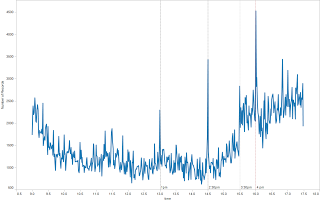
\includegraphics[width=4in]{images/shockeventtimings.png}}
\caption{Times of ``liquidity shocks'' in data from the London Stock Exchange. (Reprinted with permission from \url{http://www.anotherdataminingblog.blogspot.co.uk/2011/12/whats-going-on-here.html}.)}
\label{liqshock}
\end{figure*}

Here is an example from Dr Brierley's blog, that illustrates a algorithmic trading challenge. Figure \ref{liqshock} shows a plot made of timing of ``liquidity shocks'' in data from the London Stock Exchange -- yes, this is a really simple plot, but it tells us a lot about the data, which is:

\begin{quote}
{\em ``Now it is quite clear there is something going on at 1pm, 2:30pm, after 3:30pm and at 4pm.

Interestingly these spikes are only evident when all commodities are looked at together, they are not as obvious in any individual commodity.

My first question if I was solving a business problem would be to return to the business to get more insight in what was going on here. My initial thoughts were lunch breaks and the opening times of other Stock Exchanges around the world - as 3:30pm London time could be around opening time in New York.

Understanding the cause of these peaks is important as you would expect the reaction to them (the problem to solve) to be a function of the cause.

If we did discover it was the opening times of other exchanges, then I would ask for extra information like the specific dates, so I could calculate when these peaks would occur in the future when the clocks changed. We do not have this information at the current time, or even the day of the week (it can be inferred but not accurately as there will be public holidays when the exchanges are closed) 

As it stands any models built could potentially fail on the leaderboard (or real life) data as our model might think 2:30pm is a special time, wheras really it is when another exchange opens, or when people come back from lunch. We need this causal information rather than just dealing with the effect - time differences change - lunch breaks may change.

The current competition data is potentially lacking the full information required to build a model that is as robust as possible over time.'' }
\end{quote}

\subsubsection{Data Mining Cup}

Each year Prudsys AG  challenges students with  the Data Mining Cup competition. In 2014, the problem was announced to student team on April 2, and students needed to have their final entry by May 14. The student teams had six weeks to develop a solution for a data mining problem on the topic of optimal return prognosis. More specifically, the goal was to use an online shop? historical purchase data to come up with a model for new orders that would calculate the probability of a purchase leading to a return. In this year's competition, a team of students (Guillermo Basulto-Elias (statistics), Fan Cao (statistics), Xiaoyue Cheng (statistics), Marius Dragomiroiu (computer science), Jessica Hicks (bioinformatics and computational biology), Cory Lanker (statistics), Ian Mouzon (statistics), Lanfeng Pan (statistics) and Xin Yin (bioinformatics and computational biology/statistics) from Iowa State University was the first north American team to win. A key component of that win was the pre-processing of the data, that utilized substantial graphics to learn about their data, and inform their modeling.

Figure \ref{DMC1} shows one plot used early by the ISU DMC team, to examine return rates by time and product. Yellow indicates the ordered items were kept, blue means they were returned and pink are items to be predicted. Yes, it is a really ugly plot!!! However, it is very informative: Two major structures are immediately visible, new product introductions in July 2012 and January 2013. Themost important feature, though, is that new data to be predicted was in the third season of the time period, and this information was crucial to construct good training and test sets for model building.

\begin{figure*}[htp]
\centerline{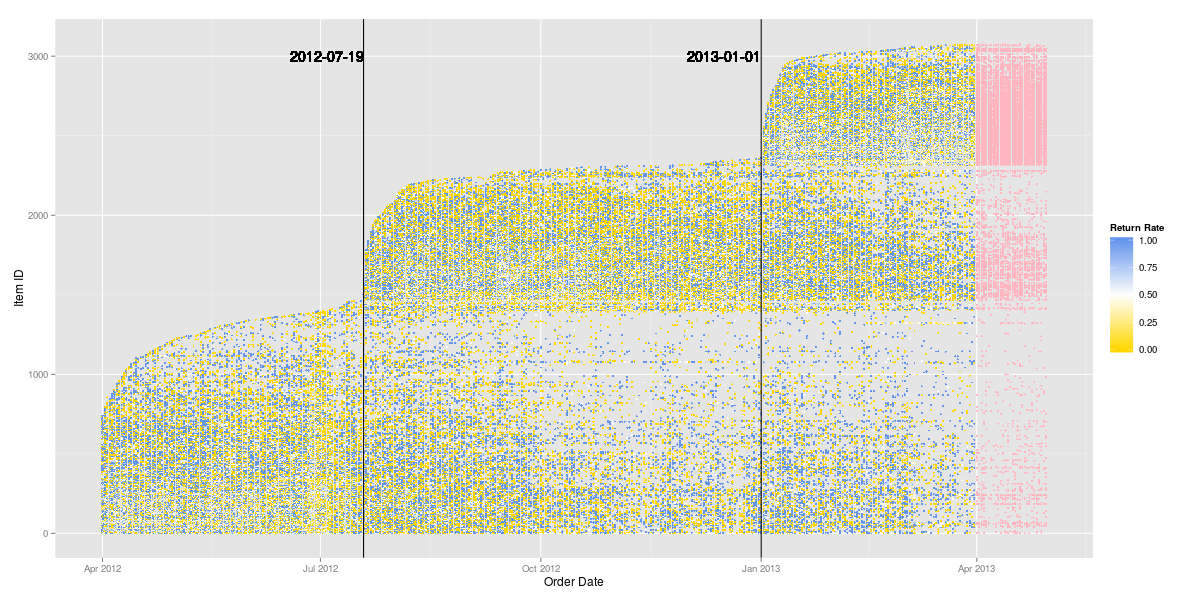
\includegraphics[width=7in]{images/orderDate_itemID.png}}
\caption{One of the preliminary plots made by the ISU DMC team. Item ID is plotted against order date, colored by return rate. The students learned that the data to be predicted (pink) did not look like the training data provided for building a model (blue/yellow).}
\label{DMC1}
\end{figure*}

\subsection{Visualization is NOT Prediction}

.... and it is beneficial in its own right. In this section, we will describe examples of visualization being used in the process of analyzing big data sets, partially from our own work and two examples from published work. What we learn from plots is different from that of modeling and prediction. 

%For big data, there are possibly many, many, many things that might be learned. There are likely many facets to the data. It is important to note that exploring big data visually is typically generating, not testing, hypotheses.

\subsubsection{OECD PISA}

The Programme for International Student Assessment (PISA) is a triennial survey conducted by the Organization for Economic Cooperation and Development (OECD) with a rotating emphasis on one of mathematics, reading, or science. In 2012, the emphasis was on mathematics. The data was made available by the OECD as part of a data challenge for the useR! 2014 conference. Entries to the competition can be found at http://beta.icm.edu.pl/PISAcontest/. 

This data is big because there is a lot of information collected in addition to the test scores. In the student table there are records for about 500,000 students from 65 different countries, and 635 variables. The variables include informaiton about gender, language, household possessions attitude to math, use of the internet, many different aspects of their lives. The parent table has 143 variables from 100,000 parent-completed surveys providing information about the students households, such as if both parents are in the home or if its a foster home, parents occupations, how the child's school was selected. The school table contains survey results completed by 18,000 school principals producing 291 variables. These items include information about numbers of teachers, supply shortages, teacher turnover, educational background of teachers, streaming of classes. There are many different questions that we might try to answer with this data. After the magnitude of the data was determined, by making quick counts of each of the tables provided, and examining the data dictionaries, our group hashed out possible questions and expectations of what associations we might see in the data.

One issue that we were interested in was about the gender gap between boys and girls in math. We hear about this in the media frequently, and we were interested to see if it is present in this multinational test data. To examine this question we calculated the diffeence between the mean math test scores for boys and girls in each of the countries, and plotted it. Sample weights were utlized in calculating the averages. The result is shown in Figure \ref{OECD-gender}. 

\begin{figure*}[htp]
\centerline{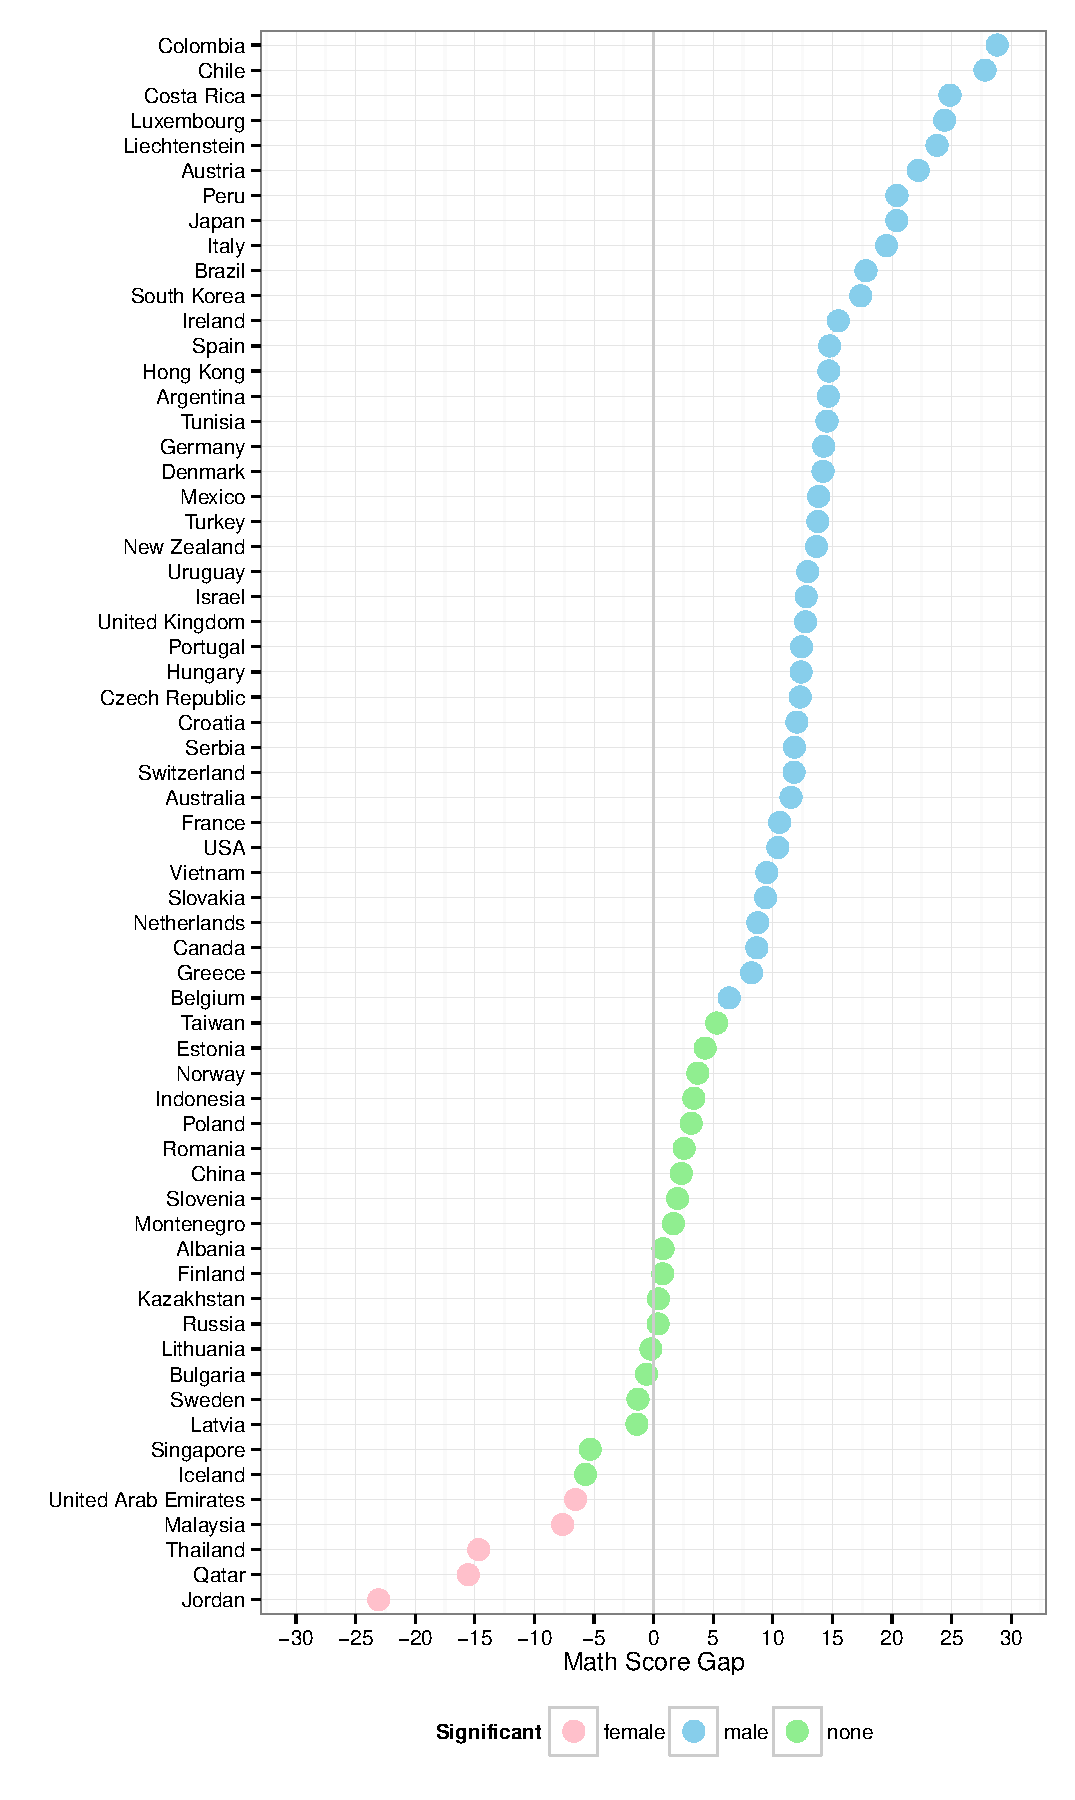
\includegraphics[width=0.5\textwidth]{images/mathgap.pdf}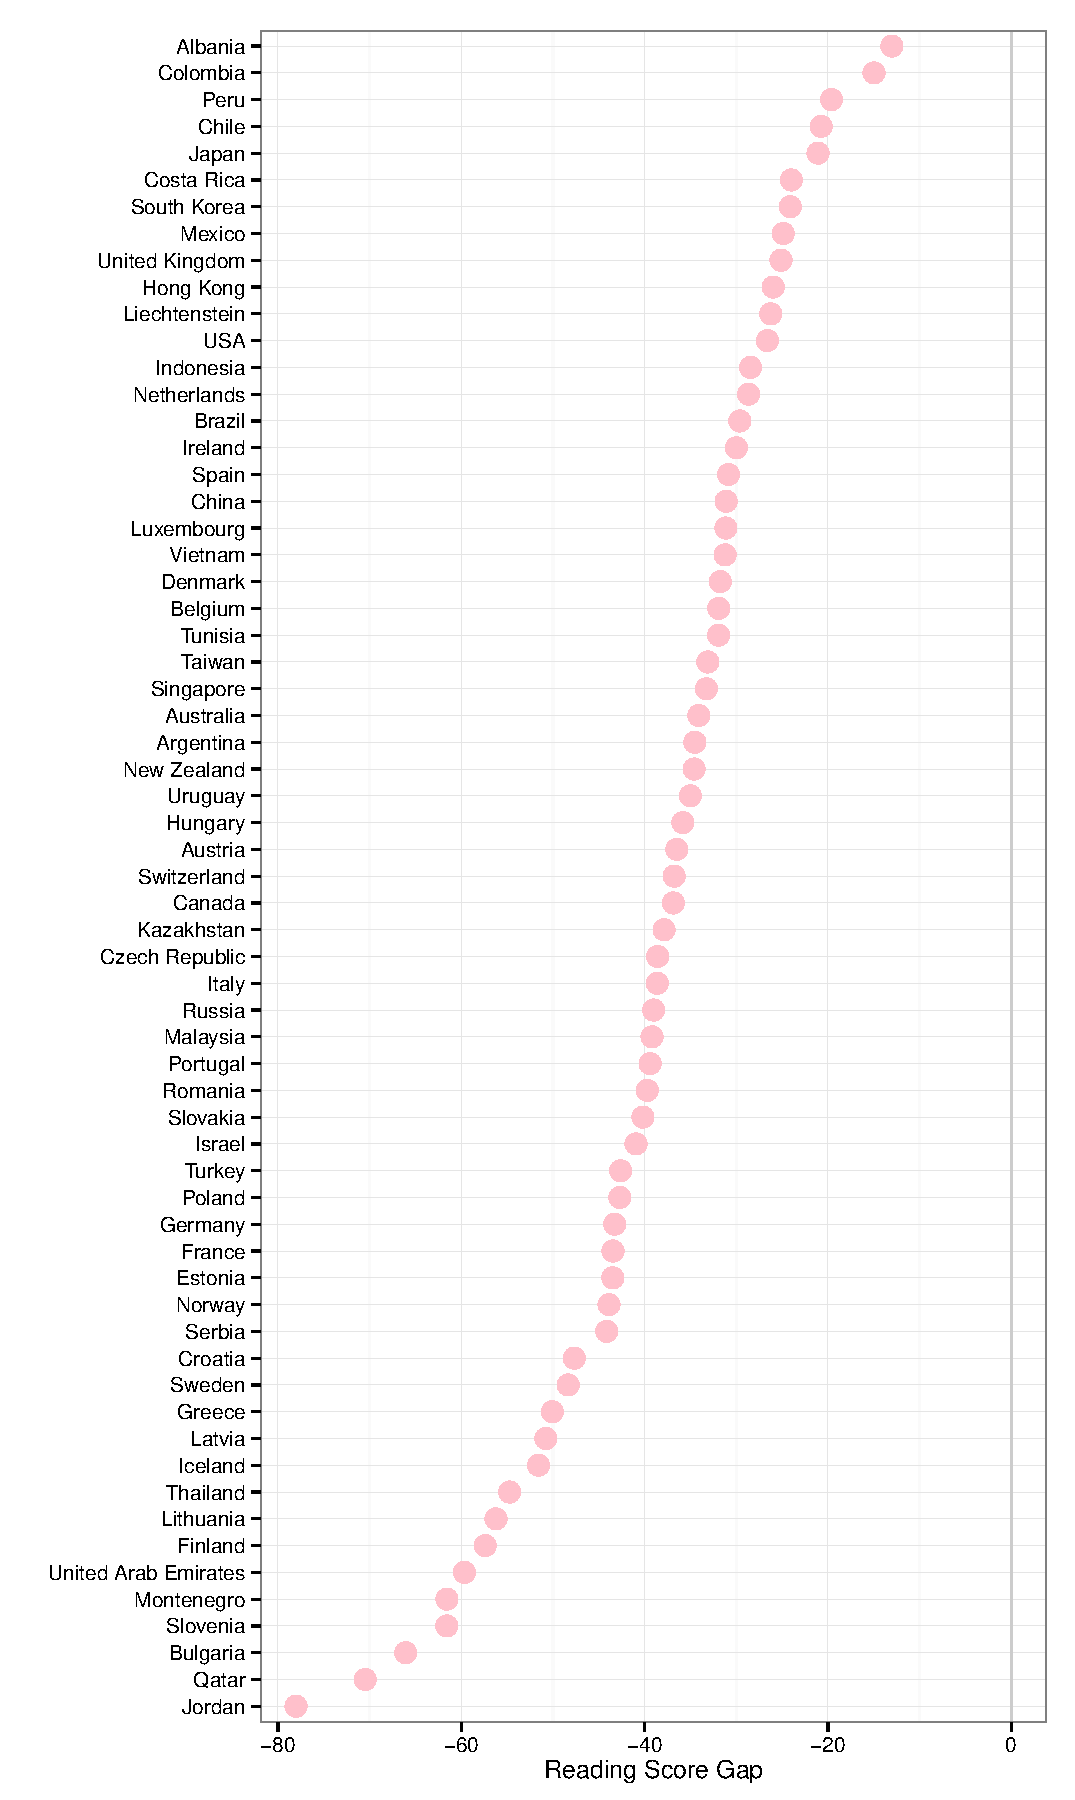
\includegraphics[width=0.5\textwidth]{images/readinggap.pdf}}
\caption{Examing the gender gap in math and reading by country.}
\label{OECD-gender}
\end{figure*}


\subsubsection{Elections}

\begin{figure*}[htp]
\centerline{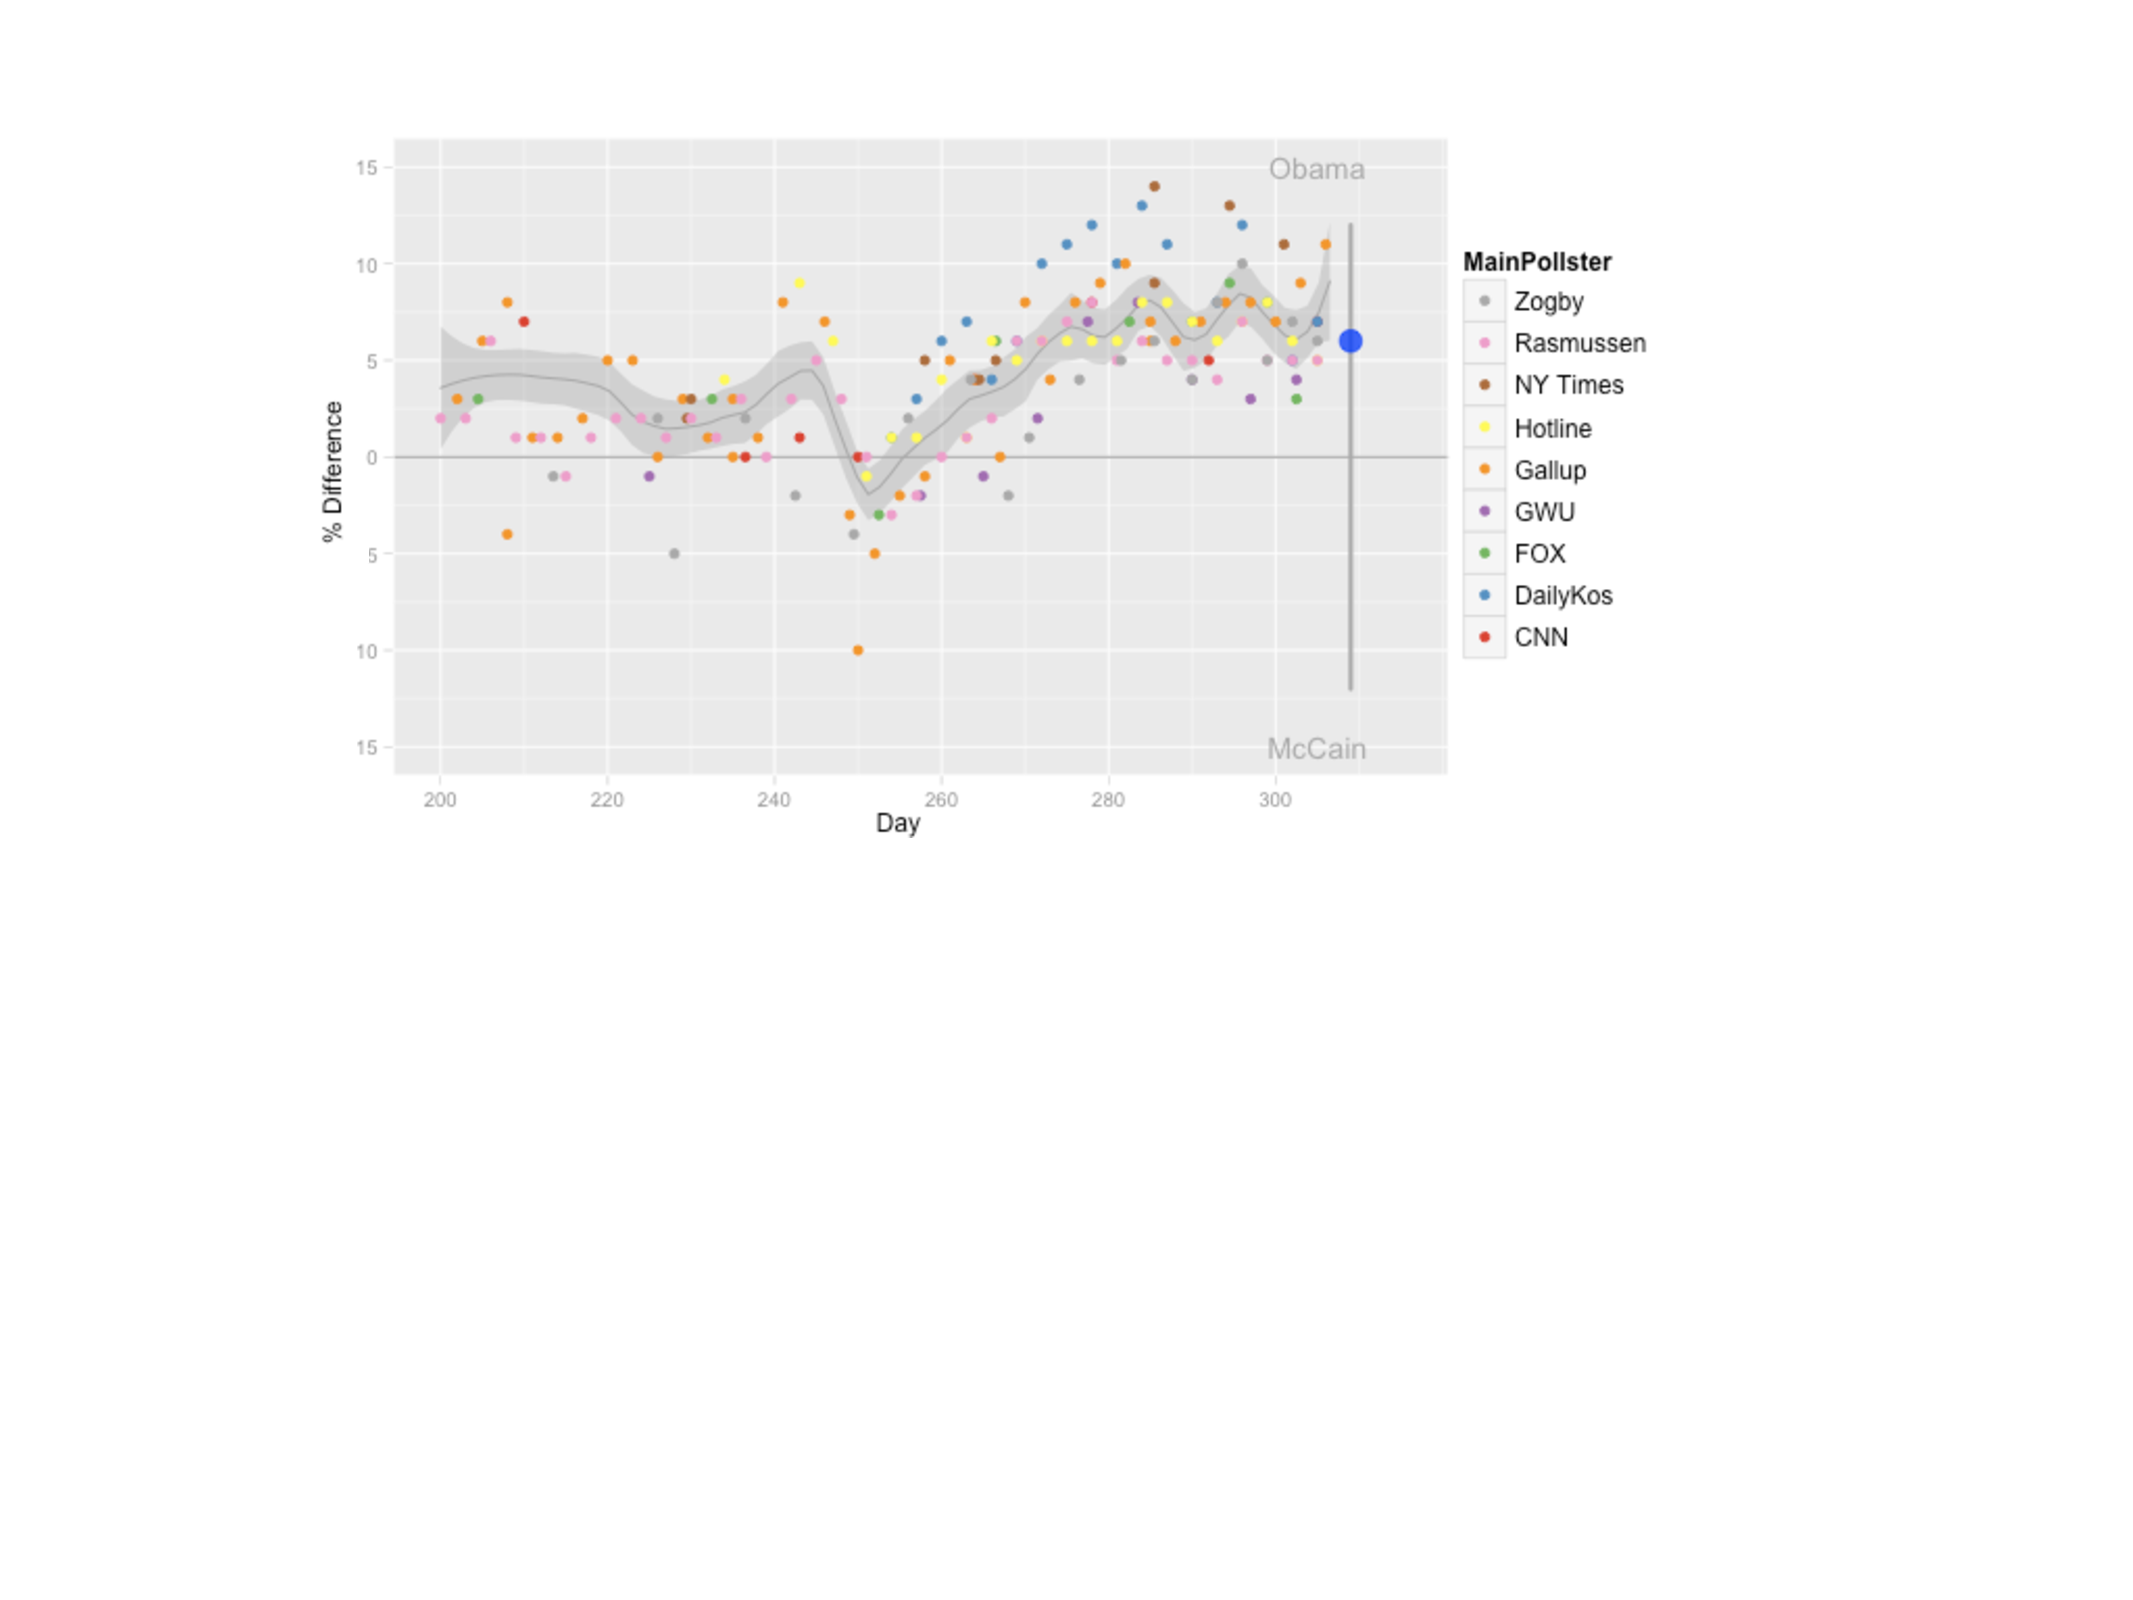
\includegraphics[width=0.95\textwidth]{images/elections.pdf}}
\caption{Tracking polls and final popular vote leading up to the 2008 US Presidential election. Percentage difference by time of poll release. Color represents pollster, gray strip shows poll average and the large blue dot indicates final election margin.}
\label{election}
\end{figure*}

In the 2008 US Presidential election cycle a young man called Nate Silver burst onto the world stage with an accurate prediction of an Obama win. His web site \url{http://fivethirtyeight.com/} (538) has expanded from politics to cover data stories in economics, science, life and sports. To obtain his accurate prediction of the election outcomes, he aggregated polls from different sources, but an important component was to adjust and weight the polls from different pollsters. Figure \ref{election} shows the polls from major pollsters, in the 100 days leading up to the election, as reported in \citet{mosley2010}. Percentage difference in percentage for Obama vs McCain is plotted against time the poll was released, as were made available on the web site \url{http://www.electoral-vote.com/}. Each dot represents one poll result, and color indicates pollster. The grey line and ribbon represents a loess smoothing \citep{CGS92} across all the poll results to indicate trend. There is a lot of variation in polls, even when conducted in very similar time frames. The variation in results can be as high as 10 percentage points. 

Differences between polls produced by different pollsters can be seen. DailyKos light blue) is consistently higher than the trend, and consistently produced the most pro-Obama results. Rasmussen (pink) tended to be fairly close to the trend or below it (pro-McCain). Hotline (yellow) was varied early on in the season but closer to election day was near the average of all other polls. Gallup (orange) is noticeably varied, it has some of the most pro-McCain results as well as the most pro-Obama results. Gallup is a legacy American pollster who dates back to the early 1900s, and we would have expected that they would be providing more reliable polling numbers than observed. Interestingly the 538 web site now has detailed ratings of the major pollsters operating in the USA, and Gallup scores a poor C+. The plot of the national trend polls allows us to see the variability and the bias' of polling organizations. The pollster DailyKos, also known as Research 200, is a community action organization with political leanings towards to Democratic party. Actually it is one of the pollsters currently ``banned'' by 538! Rasmussen on the other hand has a reputation of leaning to the right, and currently has a large adjustment value to correct this on 538. Hotline is fairly neutral. 

\begin{figure*}[t]
\centerline{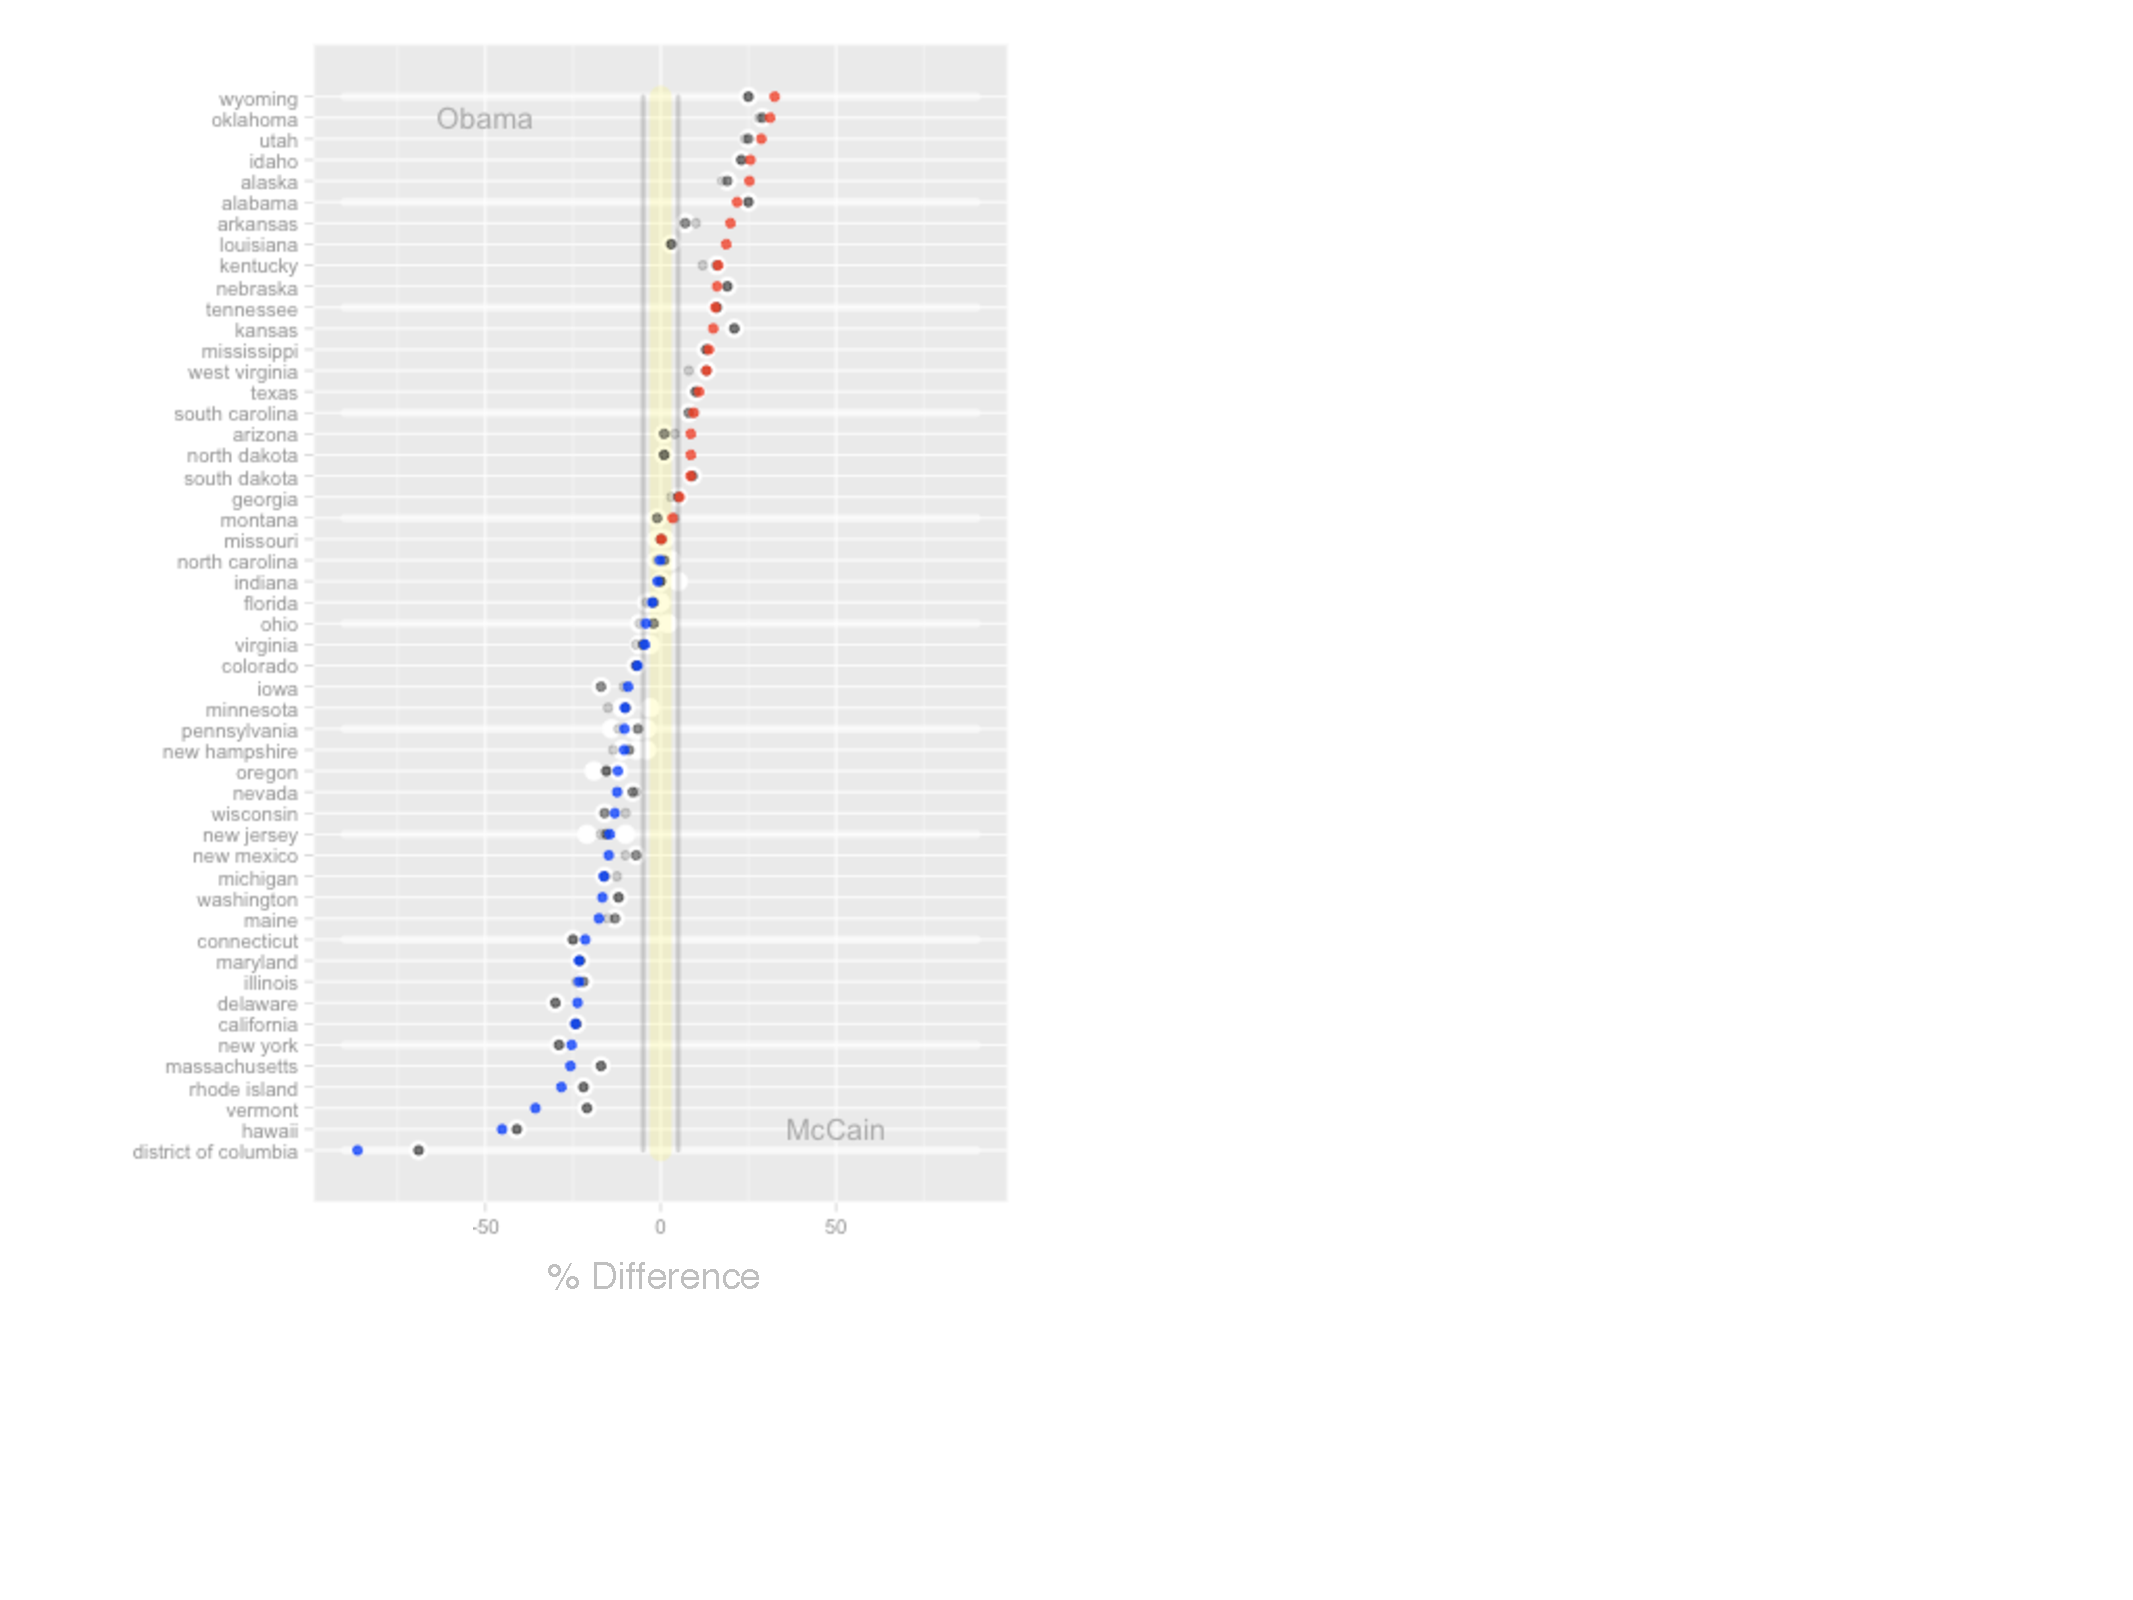
\includegraphics[width=0.55\textwidth]{images/elections2.pdf}}
\caption{Percentage difference by state, top to bottom ordered by McCain to Obama advantage. Color indicates final election result. Black is the median of all polls, grey is the median of the previous week's polls, and white shows all polls. }
\label{election2}
\end{figure*}

The US election is not won on the popular vote, though. Each state is assigned a number of electoral votes, roughly based on the size of the population. For example, in 2008 Iowa was worth 7 votes, whereas New York was worth 31. The electoral votes for most states as assigned based on winner take all: Obama won New York with 57\% in favor, so he earned all the 31 points. A candidate needs to tally up 270 or more points (of the possible 538, hence Nate Silver's web site name) to win the presidency. Figure \ref{election2} illustrates the state by state variation in polls. State, top to bottom most support for McCain to most support for Obama, is plotted against percentage difference. Each point indicates some result: the red/blue represents the final election result, black indicates the median of all polls, grey the median of the previous week's polls and white indicates all polls in that state. The yellow strip straddles a 5\% margin, with results in this range being states that are too close to call. States in these position tend to have a lot of pollsters operating, so there are more white dots visible, and for the ost part it can be seen that the final result closely matched the poll results. There are a couple of exceptions: Montana was predicting to be a toss-up but ended up being more for McCain than expected, and Iowa ended up closer than the latest polls predicted. During the election cycle, we produced these plots and animated them from the previous week, which allowed obtaining a sense of temporal shifts in attitude, and the variability leading up to the actual vote. 

In the 2012 season, this work was expanded to explore the effect of political action committee spending, after the 2010 Supreme Court decision enabled unlimited election spending by organizations \citep{kaplan2012}. And the 538 site is a fabulous location to browse for examples of numerically and visually analyzing contemporary data.  

\subsubsection{Airline Traffic}

Every few years, the graphics and computing sections of the merican Statistical Association provides a data challenge, the Data Expo (\url{http://stat-computing.org/dataexpo/}), and encourages students, faculty, industry statisticians to make a visual analysis. In 2009 the data consisted {\em ``of flight arrival and departure details for all commercial flights within the USA, from October 1987 to April 2008. This is a large dataset: there are nearly 120 million records in total, and takes up 1.6 gigabytes of space compressed and 12 gigabytes when uncompressed.''}. 

There were 9 entries, four of which won prizes, and are described in short articles. \citet{expo-wicklin} used SAS to produce a number of informtive displays about departure delays air travel in the USA: calendar view summaries show differences between years, months and days of the week, time series display volume of traffic and weekly cycles, and a heatmap is ued to compare carriers over the time period. This was a lot of data displyed very succinctly, providing key details of flight delays. \citet{expo-wickham} tackled a smaller task, comparing operations at two different airports, and \citet{expo-dey} focused on a model to find the path of least delay between any pair of airports. 

\citet{expo-hofmann} explored many aspects of the data. Maps of origin to destination show which carriers operate on a hub system and which don't. Time series of volume at major airports show effects of events like the 9/11 tragedy. Side-by-side boxplots were utilized to display delays by airport, revealing the problematic EWR, SFO, BOS, LGA and the efficient operations of DTW, MSP and DFW. Facetted scatterplots with overlaid loess fits show trends in delays by carrier. This group also looked for ``gaps'' in the data, where planes are last seen at one airport, and then magically appear at another airport. These gaps correspond to ghist flights, planes that fly passengerless, in order to get a vehicle into a locaiton that it is needed. It represents inefficiency in operations. Most carriers have been reducing this costly operation, but Northwest airlines had an increase in the latter few years of this data. Delta, which merged with Northwest in 2008, saw dramatic improvement in effciency. Basic plots revealed that many problems with the data, flights leaving 12 hours before they were scheduled, several hot air balloons that travel 430 miles per hour, and more than 200,000 flights of less than 50 miles. Stringing delays together with weather patterns revealed the problems that strong cross-winds cause at airports. And using some interpolation between geographic locations of airpots, the departure and arrival times, allowed animating air traffic flow across the nation.

\subsubsection{Wikipedia}

Wikipedia (\url{https://www.wikipedia.org/}) is a collaboratively written encyclopedia, that is a huge resource for the general public. Because it is a primary example of mass editing, the flow of edits is potentially interesting. This problem was tackled by \citet{wiki}, with an associated web site \url{http://fernandaviegas.com/wikipedia.html} where you can see some of the visualizations. The book chapter describes the process of pulling the data, pre-processing and making visualizations of different aspects. Their endeavor began in 2003, early days for the encyclopedia. As an example of the magnitude of the data, the page on ``Microsoft'' had 198 edits generating 6.3 megabytes of text, and the page on ``Cat'' had just 54 edits. 

The edits data is huge. To tackle is Wattenberg and Viega, initially created an interactive visualization for single pages. They use a modified parallel coordinate plot \citep{In85,We90}, which might also be considered to be a variation of a hammock plot \citep{hammock,ggparallel}, with versions as the variables, and text size as the stripe thickness. Stripes are colored by author, so individual contributions to pages can be tracked. (Anonymous editors are grey.) The overall height of the plot indicates the kength of the article. There are two prominent examples shown: ``chocolate'' and ``abortion''. The displays enable some information to be immediate: if there is ownership of a page by a few editors then there are a few differently colored stripes. The page for ``abortion'' has a big empty patch indicating tha the entire page was erased temporarily, probably by a malicious editor. Tug-or-wars between editors can be seen in some politically or emotionally controversial subjects. Interaction is provided to trace editors contributions and to see the actual text that was edited. 

With big data, we see that there are many different choices in what to plot. Here, the authors chose to tackle the problem using the page as a basic unit. In a secondary task their basic unit is an editor, and a new display called a chromogram is employed to enable viewing how an editor has contributed to wikipedia.  These both would be considered to be drill downs into the data, because each shows a very narrow slice of the data. There are now 4,714,447 pages, to visit each one would take some time. Ideally, approaching a problem as large as this would also provide some larger visual overviews: number of pages over time, number of authors over time, how many pages different authors edit, ... and provide some comparative views, pairs of pages for example, or hierarchical topic lists, or how pages link to each other. The data implores the analyst to display it in many more different ways. The web site \url{http://infodisiac.com/Wikimedia/Visualizations/} illustrates ways that many other people have tackled visualizing wikipedia.

\subsubsection{The San Francisco Housing Crisis}

Another book in the Beautiful series is ``Beautiful Data'' and in that volume you will find an article by \citet{SFHousing} that illustrates visually exploring the housing crisis with an early version of the R software ggplot2 \citep{wickham2009ggplot2}. This package is now almost ubiquitously used for plotting data. This book chapter is is an extraordinary example of pulling data from the web, cleaning and displaying it in different ways to learn about events that affect our lives. The explanation of the process is superb. 

The story of the housing crisis begins by studying the temporal scale: average prices and number of sales from 2003-2009. We can see the average house price double over this period, and then drop by half starting summer 2007. Sales tend to cycle some, showing some seasonality, but clear decline starting in 2006. Interestingly, sales tick up again early in 2008 after sharp declines in average price. The authors then examine economic conditions, and compare inflation adjusted,  alongside unadjusted, average price to learn that these two measures started diverging mid-2005. The two had not converged by 2009.

Breaking the data into house price deciles, and examining these relative to the median house value shows that the disparity in house prices is expanding, supporting a perspective that the more expensive houses are becoming relatively more expensive. Drilling down into each geographic regions shows that there are some areas of the city that are more affected than others: San Pablo experienced the full brunt of the boom and bust but Berkeley saw barely a hint of decline. Plotting geographicalt reveals that the eastern part of the city experienced more turnover in houses. Comparing price decline and demographic factors revealed that higher income areas, and higher percentage of college grads saw less decline, while areas where residents had longer commutes saw bigger hose price declines. 

This article illustrates elegantly how visualization can be used to explore data. 

\subsubsection{Credit card purchases}

\citet{hand2000} is an early article explaining data mining, using a large Barclay's credit card transactions database as the example. The reason to read this article is see how the humble histogram can be priceless for exploring big data. The histogram, with carefully crafted $\pounds$1 binwidth, is used to display petrol (gas) purchases, and department store spending. We might expect that in department stores there to be strong peaks just before the whole pound, and it is exactly what we see. But to see similar patterns in petrol purchases is a surprise. There are large peaks in petrol purchases at $\pounds$10, $\pounds$15 and $\pounds$20, and to a lesser extent $\pounds$12, $\pounds$25, and $\pounds$30. This behavior is driven by the consumer rather than the price points of store products -- clearly some drivers, a lot of drivers, like to spend whole nice round whole pound amounts when purchasing petrol. Beyond these peaks, the distribution looks close to bell-shaped, centered at $\pounds$20. 

Working with huge amounts of data can often be done with basic statistical graphics. There are a few cautions. Bars of small counts get lost easily with big data, which might result in failing to observe rare events. Basic scatterplots may suffer from overplotting.  Scaling up of basic statistical graphics does require some care.

\subsubsection{Text visualization}

\section{Review of the Literature}

\begin{itemize}
\item  {\tt tabplot}

http://cran.r-project.org/web/packages/tabplot/index.html

{\tt tabplot} is a R package for a visualization of a big data with various type of variables.
 All the observations are sorted by the order of pre-fixed reference variable and then divided into bins. One variable is represented by one column. For continuous variable, each bin is represented by a bar with the height of the average value in the corresponding bin. For categorical variable, the stacked bar is used.
 In this method, the big data is summarized by the binning and plotted with this summarized information for each variable. With several options, the user can change the pre-fixed reference variable,
 zoom in the specific area, or use the subset of data. Even though {\tt tabplot} allows univariate plot in parallel form, the same order of observations is used for each univariate plot and it makes the user able to compare the relationship among variables.

\item {\tt scagnostics} and ScagExplorer

http://cran.r-project.org/web/packages/scagnostics/index.html

Wilkinson, L., Anad, A., and Grossman, R.(2005).
``Graph-theoretic Scagnostics''
{\em Proceedings of the IEEE Information Visualization 2005}, 157-164

Wilkinson, L., Anad, A., and Grossman, R.(2006).
``High-Dimensional Visual Analytics: Interactive Exploration Guided by Pairwise Views of Point Distributions''
{\em IEEE TRANSACTIONS ON VISUALIZATION AND COMPUTER GRAPHICS}, {\bf 12(6)} , 1363-1372


Dang, T. N., Wilkinson, L.(2014).
``ScagExplorer: Exploring Scatterplots by Their Scagnostics''
{\em PACIFICVIX '14 Proceedings of the 2014 IEEE Pacific Visualization Symposium }, 73-80

As the number of variables is increased, the size of scatter plot matrix is getting bigger and  it is  harder to catch interesting feature from scatter plot of each pair of variables. {\tt scagnostics}(Wilkinson et al. 2005; Wilkinson et al. 2006) is developed to detect interesting features of scatter plots from the scatter plot matrix. It is started from an unpublished idea of John and Paul Tukey. It calculates 9 measures for interesting features of the scatter plot - outlying, skewed, clumpy, sparse, striated, convex, skinny, stringy, and monotonic - based on proximity in graph theory. Even though scagnostics values are calculated for the high dimensional data, it still needs to explore these values.
ScagExplorer(Dang and Wilkinson, 2014) is developed to organize scatter plots into meaningful subsets using scagnostics values. It generates several clusters of scatter plots using scagnostics values and each cluster has a leader plot. ScagExplorer uses these leader plots for visualization instead of the whole scatter plot matrix. Also it visualize the leader plots with the parallel coordinate plots of scagnostics values and use brush to select specific interesting features using scagnostics values. With scagnostics and ScagExplorer, the user can efficiently explore high dimensional data.

\item {\tt hexbin }

http://cran.r-project.org/web/packages/hexbin/index.html

{\tt hexbin} is developed for visualize two continuous variables in big data. The scatter plot is an usual way to represent two continuous variables. Because of overplotting problem in big data, it is not easy to find out the main feature of data. The main idea of {\tt hexbin} is the binning in 2D space with hexagonal bin and the counts in each bin are used to draw plot. The resulting plot is similar to the plot with alpha blending, but {\tt hexbin} is much faster than the original alpha blending. The original alpha blending needs to draw all the points with the specific transparent rate, but this hexbin method only needs to draw one point per bin and the number of bins is much smaller than the number of points in big data.

\item {\tt ggplot2} / {\tt bigvis}

https://github.com/hadley/bigvis

Instead of representing raw data with million points, sometimes it is better to summarize data in  proper way and use the summarized data for visualization. {\tt bigvis} summarize big data using aggregation and smoothing techniques. It is very useful to use before plotting big data. After summarizing big data using{\tt bigvis}, the user can draw various plots using {\tt ggplot2}. {\tt ggplot2} provides the easy way to generate complicated plots for exploring data analysis. It is developed under the grammar of graphics. It also provides multiple layers of plots that is useful to add statistical modeling results in the same plot.

%%%%%%%%%%%

\item a graphical goodness-to-fit test for dependence models in higher dimensions

Hofert M., M\"{a}chler, M. (2014).
``A Graphical Goodness-of-Fit Test for
Dependence Models in Higher Dimensions''
{\em Journal of Computational and Graphical Statistics}, {\bf 23(3)}, 700-716

Hofert and Machler(2014) proposed a graphical goodness-of-fit test for dependence models.
It is based on pairs of transformed variables with the Rosenblatt transformation. For each pairs of transformed data, Q-Q plots are generated in scatter plot matrix form. Each plot with small p-value is highlighted with different background color so the user can easily catch two problematic pairs with very large Q-Q plot matrix. All these methods are provided in R package {\tt copula}. Using highlighted background with additional information (p-value in this method), it is able to overcome the problem with high dimensional data visualization.

\item Functional Data Analysis of Tree Data Objects 23(2) 2014
Dan Shen, Haipeng Shen, Shankar Bhamidi, Yolanda Muñoz Maldonado, Yongdai Kim and J. S. Marron



\item Massively Parallel Nonparametric Regression, With an Application to Developmental Brain Mapping 23(1) 2014
Philip T. Reiss, Lei Huang, Yin-Hsiu Chen, Lan Huo, Thaddeus Tarpey and Maarten Mennes


When the number of dependent variables are very large and we need to model them with same covariates,
 the computational burden increases enormously, especially when we need to consider the penalty term with the tuning parameter. Shen {\it et al}(2014) proposed  the efficient algorithm for massively parallel nonparametric regression.
 Also they suggested the way to summarize the significant models from nonparametric regression using clustering method. With these clusters, the user can easily figure out models with similar patterns. It is very helpful for dependent data in very high dimensional space, especially for the spatial type-dependency data for example, neuroimaging data. This method is provided as R package {\tt vows}.


\item "The Generalized Pairs Plot” 22(1) 2013 Emerson JW et al.

Comment on “The Generalized Pairs Plot” 23(1) 2014 Michael Friendly

For two continuous variables, we usually draw the scatter plot. The scatter plot matrix is for multivariate variable representation. Each variable treats as continuous variable and draw scatter plot for all pairs of variables. However
the properties of variables should be considered to draw plots. The generalized pairs plot (Emerson {\it et al.}, 2013) extends the EDA idea of Tukey and allows mosaic plot for two categorical variables, side-by-side box plot for mixed variables (one continuous variable and one categorical variable). It also provides several different plots or summary statistics for all pairs of variables that the users can design the plot matrix on their own way. These generalized pairs plot are available in two different libraries in R. One is {\tt gpairs} and the other is {\\ GGally}. The approach of these two libraries are different. {\tt gpairs} is a methodological development for exploratory data analysis and {\tt GGally} is based on the grammar of graphics. Friendly (2014) suggested that this plot needs to add annotations, renderings. Also he focused on the marginal versus conditional views and and suggested to draw the generalized pairs plot with the residuals after modeling instead of the raw data itself.

\item Residual Diagnostics for Covariate Effects in Spatial Point Process Models 22(2) 2013 Adrian Baddeleyae, Ya-Mei Changb, Yong Song and Rolf Turnerd

    The spatial model is very complex model with dependent structures and it is not easy to find well-explained model. The suitable tools to check the fitted model during the data analysis procedure is very important to use. However there were no efficient tools available to check misspecification for spatial point process models.  Baddeleyae {\it et al} (2013) used the partial residual plot and the added variable plot. The partial residual plot is originally for detecting nonlinearity of independent variables in the linear model and the added variable plot is for checking the model after fitting whether new variable is needed or not. They extended these idea to the spatial point process model.  R package {\tt spatstat} is also developed for these methods.


\item visualizing high density clusters in multidimensional data using optimized star coordinates

Long, T. V. Linsen, L.(2011).
``Visualizing high density clusters in multidimensional
data using optimized star coordinates''
{\em Computational Statistics}, {\bf 26}, 655-678

After the cluster analysis, we need to check the distribution of clusters, the relation or distance between clusters, etc. However if we have very high dimensional data, it is not easy to check these points visually. Long and Linsen (2011) propose the visualization method for a hierarchical tree of high density clusters in high dimensional data. They project the multidimensional clusters to a 2D or 3D layout using an optimized star coordinates layout. It allows to explore the distribution of clusters interactively and help the user understand the relations between clusters and the original data space.

\item OnSet

Sadana, R., Major T., Dove, A., and Stasko, J.(2014).
``OnSet: A Visualization Technique for Large-scale Binary Set Data''
{\em IEEE TRANSACTIONS ON VISUALIZATION AND COMPUTER GRAPHICS}, {\bf 20(12)} , 1993-2002

When one observation is a set of elements, we can make the whole list of elements from all observation and dataset is rearranged that each elements represents binary variables and if one observation has the elements, get 1 as a value, else the value is 0. if the whole list of elements are very large, it is not easy to figure out the features of data.
OnSet is a technique to visualize large-scale binary set data. One observation is represented in one layer of plot and one pixel represents one elements in the plot. For the elements in this observation, pixels are highlighted. With these type of representation, it is easy to calculate "and" ,"or" operations.


\end{itemize}

epivizir

\section{Technological Advances}

\section{Synopsis}

Explain working definitions of terms related to data visualization: infographics, information visualization, visual analytics

Talk about fishing! And avoiding fishing. And Buja's post-model ...

What I'd like to do for the big data visualization review paper is to focus on the importance of plotting data to learn things that were not expected, and to improve data analysis and modeling.

\begin{itemize} \itemsep 0in
\item Very short intro to the spirit of EDA, as was practiced by J. W. Tukey.

\item How technology has changed the landscape of EDA

\item Work that has come between Tukey and the young researchers of today, focusing on people who may not have received a lot of attention: Andreas Buja, Antony Unwin, Chris Wild, John Maindonald, Debby Swayne, Hadley Wickham, Yihui Xie.

\item What are the building blocks for his successors today: R and bioconductor, enable everyone to participate; reshaping data, data wrangling, split-apply-combine,

\item The largest chunk will be examples from people who have won major big data analysis competitions in the past year, how visualization played a role,  what plots they made and what they learned from them, that helped to improve the model results.

\item Interplay between exploratory and inferential statistics, how to couple discovery of structure with assessment of how real the patterns are.

\item Also will review relevant publications in major journals: TAS, JCGS, Computational Statistics, Statistical Science, JASA, JSS, ... that show new graphics methodology.

\end{itemize}

\bibliographystyle{asa}
\bibliography{visualization}

\end{document}

% John Deere, Andy Roberts

% Data Mining Cup team

% Phil Brierley


